\section{Das Modell}
Im folgenden Abschnitt soll das in \ref{fig:ccmodel} gezeigte Modell zur Beschreibung von DNS-Cloud-Services detailliert erläutert werden. Dies soll zum Verständnis und als Hilfe bei der Anwendung dienen. Außerdem soll es die gewählte Darstellungsform und Notation beleuchten, die zur Erstellung des Modells genutzt wurde.

\begin{sidewaysfigure*}[ht]
    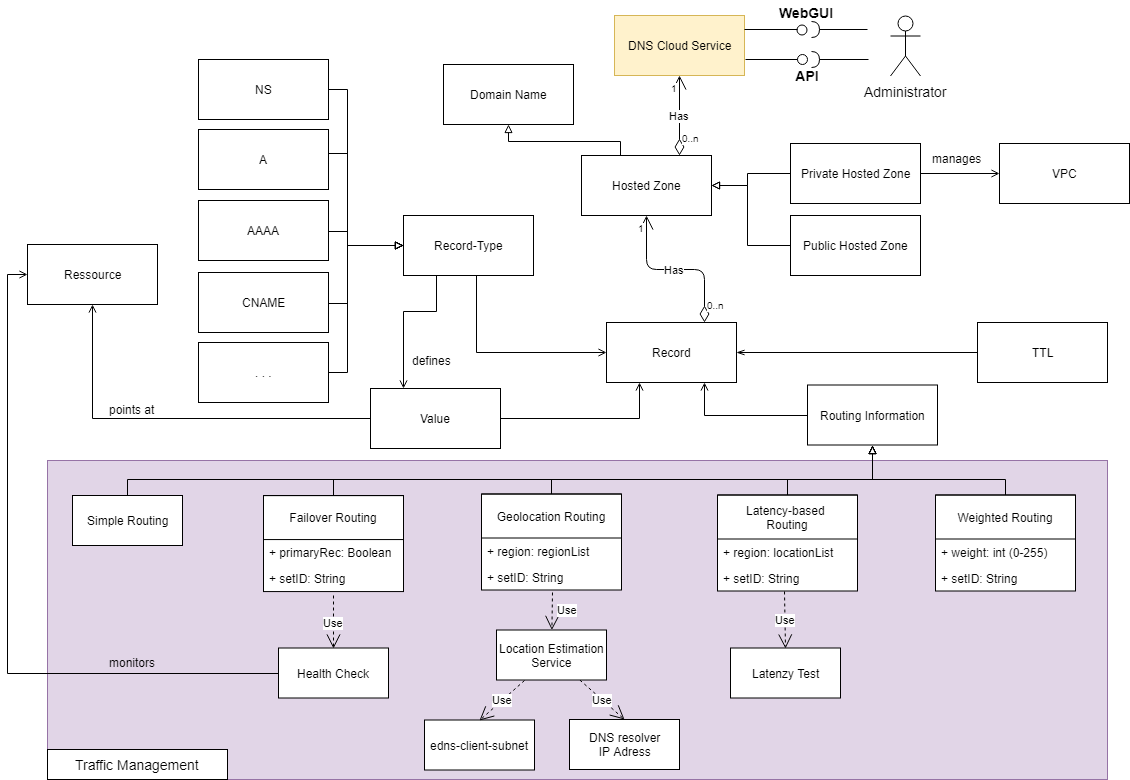
\includegraphics[width=\textwidth]{images/cc_modelxml.png}
    \caption{Modell zur Beschreibung von DNS-Cloud-Services}
    \label{fig:ccmodel}
\end{sidewaysfigure*}

\subsection{Schnittstellen}
Zur Nutzung der DNS-Cloud-Services stehen unterschiedliche Möglichkeiten zur Verfügung. Wird ein neues Benutzerkonto angelegt, geschieht dies über eine Weboberfläche. Nach der Einrichtung ist es möglich über die Benutzeroberfläche der Internetseite auf das Produktportfolio des Dienstleisters zuzugreifen. Sämtliche Interaktionen mit dem Cloud-Service sind über diese Weboberfläche möglich. So kann der Kunde jederzeit und von jedem internetfähigen Gerät, plattformunabhängig über den Browser seines Betriebssystems auf die Services zugreifen. Das bedeutet, dass keine Installation von zusätzlichen Anwendungen oder Treibern notwendig ist.

Eine weitere Möglichkeit ist der Zugriff über eine Schnittstelle zur Anwendungsprogrammierung (API). Diese Schnittstellen ermöglichen es über Kommandozeilenwerkzeuge auf die Services des Cloud-Providers zuzugreifen. Somit können auch ohne die Hilfe des Webinterfaces  administrative Aufgaben bezüglich der Cloud erledigt werden. Des Weiteren ist es möglich über Skriptsprachen Routineaufgaben zu automatisieren oder den Cloud-Service in eine unternehmensinterne Software einzubinden. Dies bringt den Vorteil eines flexibleren Umgangs und einer bessere Einbindung des Cloud-Services in die alltäglichen Prozesse.

 \subsection{Hosted Zones}
 